\documentclass[10pt,oneside,english,a4paper]{article}

\usepackage[T1]{fontenc}
\usepackage[utf8]{inputenc}
\usepackage{graphicx}
\usepackage{url} 
\usepackage{hyperref} 
\usepackage{cite}
\pagestyle{headings}
\usepackage{indentfirst}

\title{How to get  to get the collaborative work skills through E-Learning\thanks{Semestrálny projekt v predmete Metódy inžinierskej práce, ak. rok 2020/2021, vedenie: Ing. Fedor Lehocki, PhD.}} 

\author{Polina Kubyshkina\\[2pt]
	{\small Slovenská technická univerzita v Bratislave}\\
	{\small Fakulta informatiky a informačných technológií}\\
	{\small \texttt{xkubyshkina@stuba.sk}}
	}

\date{\small  15. november 2020} 

\begin{document}

\maketitle
\begin{abstract}
In the past years the attitude toward the idea of e-learning has drastically changed. The idea of getting knowledge on-line does not seem that surprising any more. But when it comes to on-line learning is it possible to get practical skills on-line? Is it possible to teach people to communicate with each other and be able to work in a group with somebody through the e-learning?\par
This paper examines how people usually get the collaborative work skills and makes pattern for teaching it via the digital technology. A survey is put to see if people even see the need in such skill nowadays. The results are analysed from the different prospective to answer the question stated in the title.
\end{abstract}

\section{Introduction}

In the past year the term ``E-learning`` has become more widely used than ever before. The events happening in the world forced humanity to think about organizing the studying without the physical interaction between the teacher and the pupil. The ``E-learning`` itself has provided us with the idea of getting any possible information via Internet. It has opened a lot of paths for thousands of people, but at the same time it has brought to life several problems that need to be solved. The article ``Improving e-learning to meet challenges in 21st century`` published by Dilrukshi Gamage, Indika Perera and Shantha Fernando brings up the doubt about being able to get important practical skills through the e-learning methods.\cite{collab2} Generally, because of the fact that E-learning doesn`t really require constant face to face interaction, it suffers from the lack of group base learning, meaning that people don`t interact with each other and don`t know how to work in collaboration with others. It results in not being able to collectively solve the problem or the task. The other source ``Developing Active Learning Experiences for Adaptive Personalised e-Learning`` also focuses on this problem and the possible solution – a specific organization of E-learning and collaborative learning to overcome this problem.\cite{collab1}

\section{The Definition of E-learning} \label{definition}

E-learning – a term that came into our lives recently, but in the past year has taken its place in the educational environment. Modern reality has forced everybody without any exceptions to put their minds to it and, to a certain extent, to learn how to use it. But for a regular person this term is still not fully understandable, so firstly it`s important to define it.\paragraph{}
According to the Oxford University dictionaries the e-learning is typically learning that is distributed through the electronic devices, in most cases via internet. Similar definition can be found in the Cambridge dictionary. They also add that this type of learning is done at home using computers.\paragraph{}
But there is also a separation within this term. The two approaches that currently exist are learning through and using technology. First one means that technology-enhanced learning is the only way of learning used, while ``learning using technology`` is more about technology being one of the many learning methods, but not the only one. For this article we will use the first approach, as the second one is usually not the one people think about when they hear the term ``e-learning``.

\section{Collaborative skills} \label{collab}

It’s a well-known approach that one of the missions of school is to teach children or more officially students to be able to communicate with each other. In the past several years this idea has been moved backwards and is not currently considered as important as it used to be. People become more and more self-centered and communication itself loses its` importance. But when it comes to working in groups it`s highly important to be able to communicate with your group partners, other wise the collaborative work is no longer ``collaborative``. The absence of the communication skills highly affects human`s ability to work in group and collectively solve the stated problem or task. This is where the idea of getting collaborative work skills appears.\paragraph{}
Firstly, it’s important to define this term too, as there are many different definitions applied for it in several scientific fields. Generally, collaboration is the idea of working on something together in order to solve a certain problem. But a deeper perspective into what it is can only be the key to fully understanding what ``collaborative work skills`` means. For example, in 2019 as a second year software engineering student I got a task to create a software system in a group with my group mates. The possibilities were endless, so we started thinking about what we wanted to create. As ambitious as we were back then we decided to make a PC game. But when it came to making decisions about certain details of the project that`s where we got stuck. Everybody had his own prospective on the final result and the ways of its achievement. The main reason for this was that nobody was ready to listen to his opponent and consider his idea as a possibility for the project topic. What I am trying to state here is that the first and main feature of collaboration is the ability to listen to other people. And not only listen but also to hear what they`re saying. Secondly, it`s important to be able to consider other ideas besides your own and be able to admit them. It`s leads to realization of the main goal of every group activity – achieving a certain goal, where the group result is important and not the somebody`s personal goal achievement. Work in a group is like a mechanism where nothing would work without participation of all of the parts.

\section{Current Approach} \label{curr}

In the modern world the idea of traditional organization of work and study is slowly coming to its logical finale, the priorities change with the development of the world wide web. More and more organizations replace the traditional office environment with the virtual office. The majority of organizational work is moved on-line. But the tasks remain the same. People learn how to solve them in the new reality. But as for the younger generations for whom it is almost natural to live ``on-line`` the situation is different. All the practical communication skills mentioned before for these younger generations are something that seems not as important. What is stated here is not that children do not know how to talk to each other, it is more about them not being able to solve the task in cooperation with others. It is not something that is learned naturally throughout life, but something which requires some specific training, which is usually provided by schools, then universities. \paragraph{}
Modern e-learning system focuses on giving children study material, organizing exercises and giving test to see if the material was successfully understood. But it does not focus on building the relations between students. 

\subsection{Statistics} \label{stat}
To understand the current situation more a survey was held among 48 respondents from 6 countries. The purpose of this survey was first of all to define the importance of getting the collaboration work skills and see if people who spent the majority of their life studying and learning traditionally obtain the following skill. It's important to note that 80,9 \% of the respondents are from the age of 18 to 24, 12,8 \% - from the age of 25 till 30 and only 6,4 \% older than thirty. Among the ones who passed the survey 44,7 \% are current students. Statistically speaking the results would mostly reflect the views of current students getting the bachelors or the masters degree, so they will be considered the majority group. 

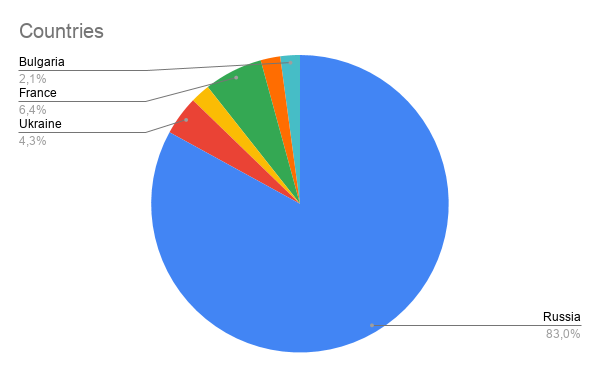
\includegraphics[width=0.7\textwidth]{Countries.png}

Almost all of the respondents said that it is essential to have collaborative work skills, which gives the right to conclude that in the modern world people still value the communication and the ability to communicate, or more over also to hear and listen. Also it is possible to conclude that even the digitalization and converting all the work to the on-line format don`t cancel the need to collaborate. People are not physically in one place but still perform the work collectively.

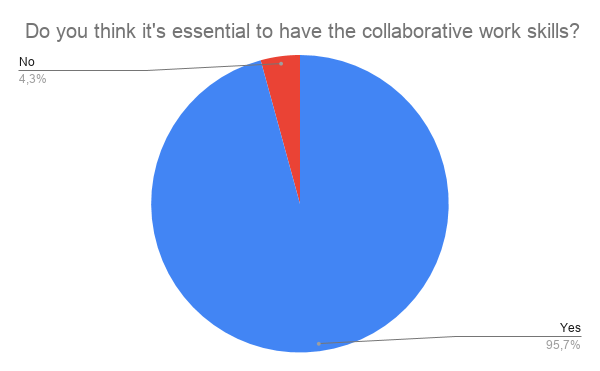
\includegraphics[width=0.7\textwidth]{diagram2.png}

Next question was aimed to see if people consider the possibility of solving a task in a group on-line. The majority of respondents answered positively. 

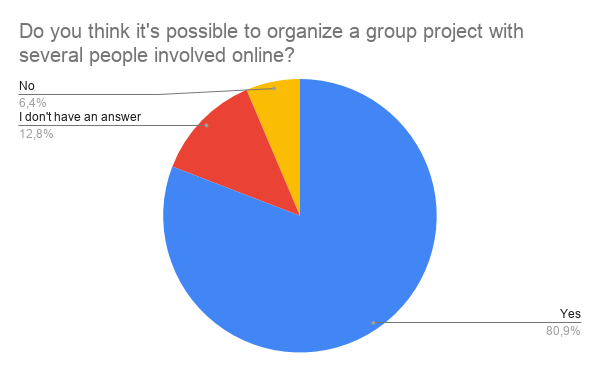
\includegraphics[width=0.7\textwidth]{diagram1.png}

Regarding the question about if it is convenient to solve tasks requiring collaboration on-line opinions divided equally. It's important to note that among the respondents aged 25 and older only one person has said that it would have been more convenient for him to work on-line. The majority of respondents from this age group still answered negatively. 
Among the respondents younger than 25 the reaction was completely the opposite. 

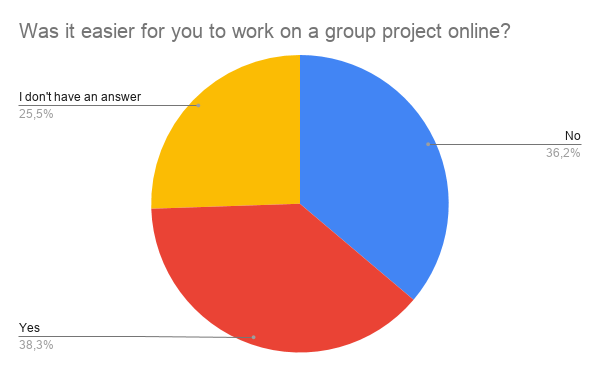
\includegraphics[width=0.7\textwidth]{group_work.png}

However, when the respondents were asked about the whole process of education and possibility to transfer it on-line, people were not as positive about it. Only 23,4 \% said they consider such option. The majority still answered that they would prefer the traditional way of education. When they were asked to specify the reasons why they don't consider such options 30,3 \% said that the practical skills cannot be learned through the digital devices. Some even specified and pointed out the idea of getting the skills of working in a group. 

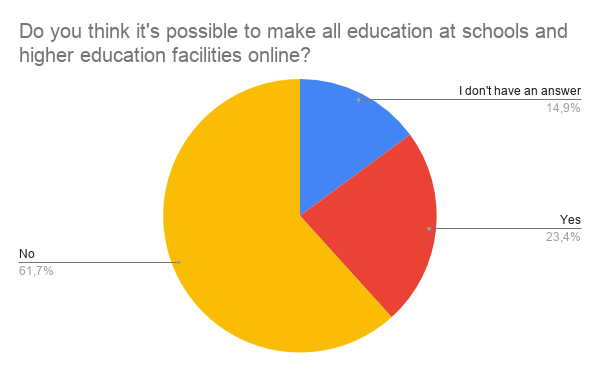
\includegraphics[width=0.7\textwidth]{diagram3.png}

\subsection{Analysis} \label{analysis}

It may seem that the survey results don't make any sense, as the survey itself is not about getting collaborative skills, but the purpose of this survey was, first of all, get an answer to the question: "Is it important to have collaborative work skills nowadays". It may sound trivial, but with digitalization and changes in the daily life and work, many functions and skills lose their purpose and become, in a manner, atavisms. Lets take the skill of memorizing big amounts of information, for example. In the 21st century every person has access to the endless amounts of information of all possible kinds. It's not hard to find it, if needed. Several clicks and the result is displayed on the monitor. There's no need to memorize information. Several decades ago such information could be only accessed by books, which were not so easy to get, and it took quite some time. Perhaps, the results of the survey showed that the modern generation still considers this skill essential. \paragraph{}
The next question, we need to get an answer to by sublimation of the survey results is "How convenient do people consider solving group tasks on-line". Although, the equal percentage of people answered negatively and positively to this question, there's also a category of people were indifferent about this question. This means that even despite the digitalization modern generation is still not ready to move all the group activities on-line.\par

\section{Current eduction standards} \label{back}
Modern educational standards use certain teaching methods that are organised differently and focus on different aspects of human psychology.  Generally all of them can be divided into two categories: teacher-centered and student-centered.
\subsection{Modern teaching methods}
\begin{table}[h!]
  \begin{center}
    \caption{Teaching methods}
    \label{tab:table1}
    \begin{tabular}{l|c|c|r} 
      \textbf{Teaching method} & \textbf{First appeared} & \textbf{Teacher}& \textbf{Requires self-research}\\
      \hline
      Lecture-based learning & - & Authority & No\\
      Flipped classroom & 2007 & Authority & No\\
      Adaptation learning & 1970s & Authority & No\\
      Inquiry-based learning & 1990s & Mentor & Yes\\
      Game-based learning & 2010s & Mentor & Depends\\
    \end{tabular}
  \end{center}
\end{table}
\subsubsection{Teacher-centered methods}
Teacher-centered teaching methods obviously put the teacher as the head of the process in every aspect. Teacher is the one who instructs and shares the information, and the students are the "Empty vessels". \cite{vessel} From this point of view the information as an object is transmitted from the teacher to the student. \paragraph{}
First of all, we have the "Lecture style"  teaching method which focuses one-way communication, where teachers and students are not involved in any sort of communication. Professors read their lectures and give assignments. Students listen to lectures and do the assignments. The discussion barely exists in this type of teaching. The whole teaching process is based on teachers giving instructions and students learning through following these instructions.\paragraph{}
The second teaching method that has appeared pretty recently but has already gained popularity among some social groups is the so called "Flipped classroom" method".\cite{Flipped} As it is being said this method is basically the opposite to the standard "Lecture" style method. It's idea is that the lectures that are traditionally held off-line are prerecorded and sent to the students. The  assignments on the other hand are done in the classroom. \paragraph{}
One more teaching paradigm that exists but is not commonly used is the "Adaptation" method.\cite {Learning} This paradigm is based on the idea of "learning styles". Basically all human beings process information better through the certain perception channels better than through the others. This means that for someone it's easer to learn something through listening to it, while for his best friend it's a lot more convenient to look at the book while memorizing information. 

\subsubsection{Student-centered types}
Student-centered types on the other hand put students and teachers on the same line. Both of these categories now play the equal role in the learning process in terms of importance. The teacher is considered to be more of a mentor who guides rather than tells exactly what to do.\paragraph{} 
One of the methods that uses this approach is the so called "Inquiry-based learning" method.\cite{inquiry} It's idea is for the students to create the inquiries based on their research on the topic and get involved into the topic through this. This method requires a deeper level of investigation from the student rather than the teacher. \paragraph{} 
Another method that has been gaining more and more popularity recently is "Game-based" learning. The whole idea here is to teach through games, as simple as it seems. This method relies more on teaching soft-skills such as the ability to solve the problem by analysing the given circumstances. This method is also a logical conclusion of the whole love for games in the modern society.

\subsection{Stating the problem}
Different teaching methods that are stated in this article have been in use for a while and were generally developed to teach students under normal circumstances. The global pandemic has changed all life aspects, and education is not an exception. \paragraph{} 
The standard teaching methods the way the used to work before can no longer be applied to education. Everything needs to be modified to meet the new reality. And, if we are talking about standard theoretical skills this doesn't seem to be a problem, more of an advantage. With practical skills situation is the opposite. Collaborative work skills and e-learning don't seem to cooperate very well. So the purpose of this paper is to suggest the possible solution on how to incorporate teaching this skill into the teaching of the pandemic.

\section{Using the technology to develop practical skills}
 \label{chan}
Generally, the answer is pretty clear - to use technology. But, if we try to specify things no longer seem this easy. First of all, how can e-learning support collaboration projects? How can teachers evaluate collaborative work and give feedback to it? \paragraph{}
In the next chapter I will suggest a possible way of organisation of education that will be able to full fill the all the requests and solve all of the stated problems.
\paragraph{} 
Overall, learning a skill is like a logical function, which takes two or more parameters and returns a  boolean result. So the skill is either obtained or not. This is the only possible way to evaluate it.  In this article the two taken parameters would be the teaching method and the technological support.
\subsection{The particular teaching method}
Even though people have been trying to gradually incorporate technology into education for the past several decades no one has ever thought we would have to implement it in less than half a year without any testing. The tests are being held along side with teaching. And even this short time period has shown that the standard teaching methods can not show the positive results, they need to be modified to fit the modern reality. \paragraph{}
Since this paper doesn't focus on teaching in general we would not speak about the effectiveness of teaching methods regarding the theoretical knowledge. The idea is to find the method that would be able to teach the students how work collaboratively. When at the learning facilities these skills can be obtained natively and gradually even without the specific teaching, but now when people's private rooms become their classrooms this scenario doesn't work. And so doesn't the traditional "Lecture-based" teaching method. The idea of blind learning doesn't require basically any communication and critical thinking. The idea of the "Flipped classroom" doesn't work either for the same reason. Here changing the order of the addends does not change the sum. Just like Dr.Aaron Barth stated in his speech for the TEDx Talks the key to successful  learning is creating empathy and engagement. The idea of so-called "Story-based learning".\cite{barth_2020} Learning that doesn't teach to think according to the knowledge but think outside of the stated borders. This thesis is implemented in some of the teaching methods that were stated in the previous chapters to a certain point. For example, "Game-based learning". Games are a very powerful instrument that can in an interesting manner make people think or create engagement. Exactly what is needed. The same also works for the "Inquiry-based learning". Questions lead to investigations which lead to critical thinking. 
 
\subsection{How to incorporate this into e-learning}
How can this be implemented in the idea of getting collaborative work skills? Well, it's scientifically proven that in order to get a skill it needs to be constantly practised. Engagement in the topic is the first step to discussion.  \paragraph{}
Other problem regarding this is how to build a discussion through the e-learning? Just like it was previously stated the key here is to choose a specific teaching method and a certain technological solution in order to replace the traditional in-classroom education and a create a space to communicate and collaborate.
\subsection{Technological solution}
The statistic survey results have shown that collaborative work is still very popular and is widely used. In the era of technology people have created multiple technological solutions in terms of collaborative work. \paragraph{}
First and, probably, most popular one is "Trello" - a cloud program built to control the projects. It's idea is to create boards to see the roles of each group member and the steps the project realization is broken into. But this app does not focus on collaboration in a way that we are currently speaking about. It relies more on the technical side of the topic. It's helpful to delegate the work within the team but not to build the collaborating skills.\par
\begin{center}
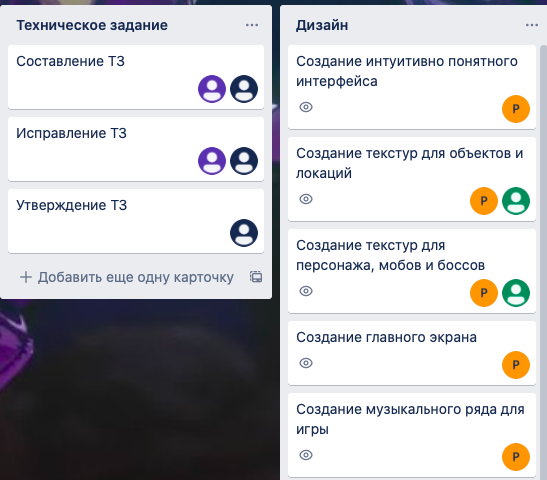
\includegraphics[width=0.7\textwidth]{Trello.png} 
\end{center}
Team communication can be reached through the messengers but the problem with this is that having many tools only makes things more complicated and usually leads to the opposite to expected result - not being able to collaborate. \paragraph{}
The solution could be putting everything in one place: messenger, tables, notes. Creating the virtual conference room where people can work together and share their work and progress through the different channels. Certain apps already have this feature implemented to the certain extent. For example, let's look at "Axure" - a well known prototyping system. It has a feature, called the "Axure Cloud" - a cloud solution that allows all the members of the group to modify the project, comment and communicate within the app. 
\begin{center}
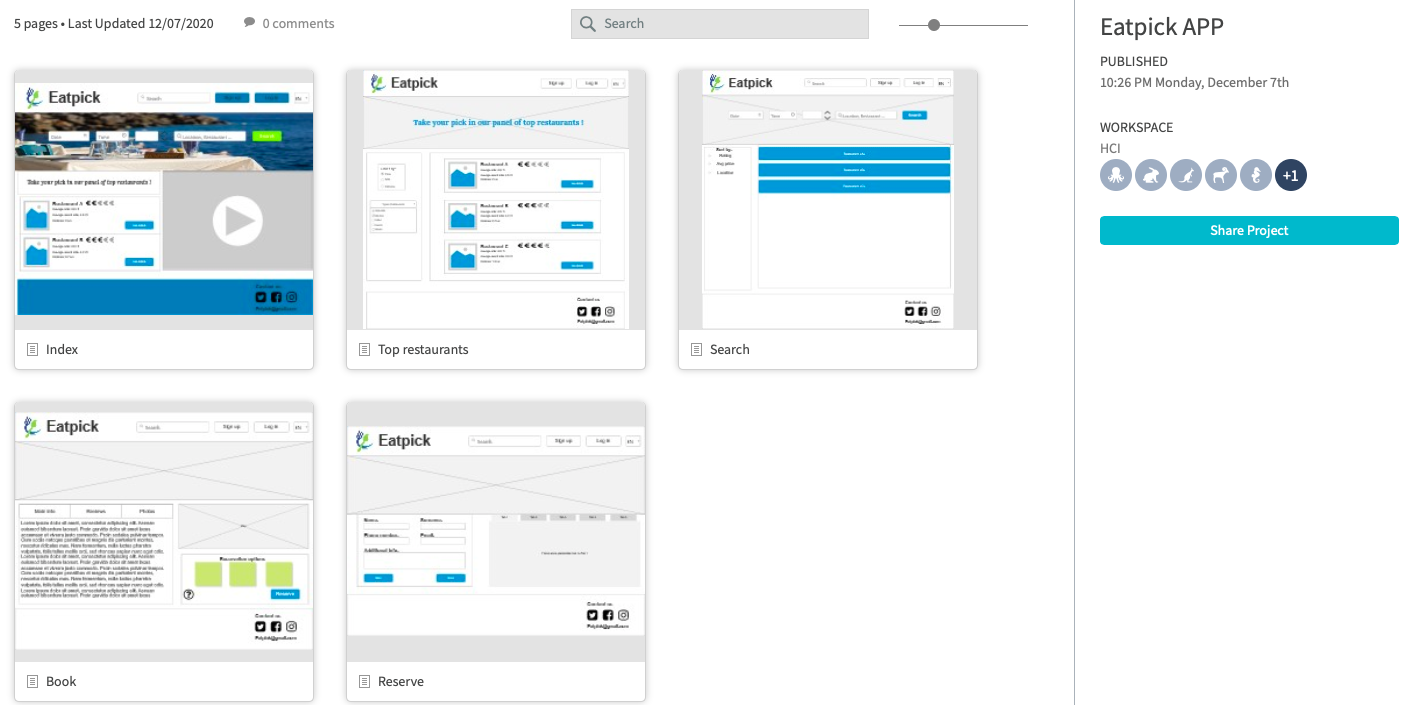
\includegraphics[width=0.7\textwidth]{Axure.png} 
\end{center}
\section{Conclusion} \label{zaver} 
The idea of this paper was to suggest a possible way of getting the collaborative skills through e-learning platforms, to find the suitable "x" and "y" for this mathematical problem. In order to prove it a deeper research should be done, but as a thesis this creates the platform for further investigations as there can be multiple suitable solutions. \paragraph{} 
The idea of two parameters for learning the skill is very simplified but it generally reflects the idea this paper gives. In order to organize learning collaborative work skills two things are required: specific engaging teaching and evaluation methods and technological solutions meeting the criteria for the successful collaboration.

\bibliography{literature}
\bibliographystyle{plain} 

\end{document}